\section{\Model}
\label{sec:approach}

\begin{figure*}
  \centering
  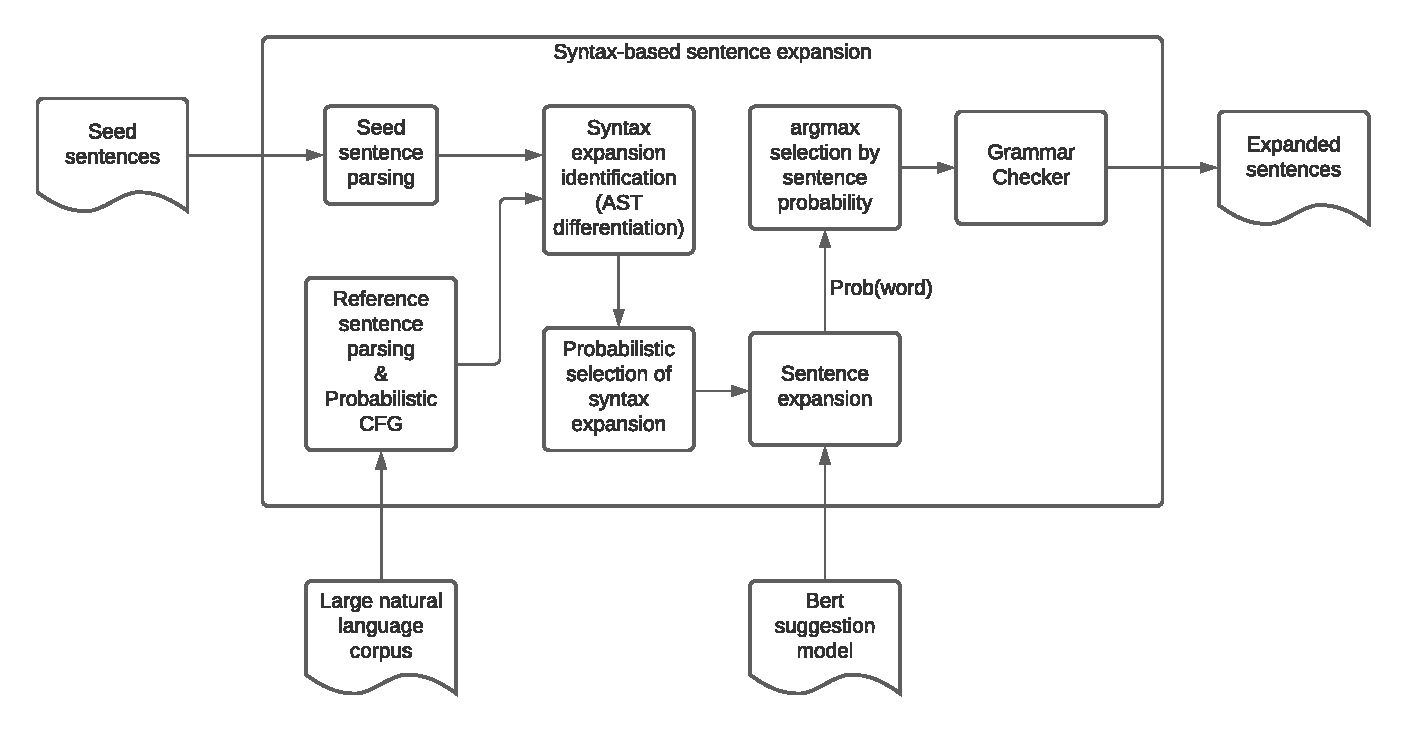
\includegraphics[scale=0.5]{figs/overall.pdf}
  \vspace{-5pt}
  \caption{\OverallModelFigCaption}
  \vspace{-10pt}
\end{figure*}

This section presents our architecture of \Model for generating input
sentences. The high level of \Model is illustrated in
\ref{fig:OverallModel}. \Model first searches seed sentences that
meets each requirement for a linguistic capability. The seed sentences
are parsed into their \cfg. Meanwhile, \Model builds the reference
\pcfg from a large natural language corpus. Each \cfg of seed
sentences are 
